
\textbf{NOTA: Las figuras de este capítulo son temporales.}


\section{Introducción}
Una secuencia de pulsos se refiere al orden cronológico y las características de cada uno de las manipulaciones que se hacen a un sistema de spins con el fin de producir una señal interpretable. En el caso de la realización de una imagen, se refiere a la temporalidad, orden, y parámetros de la manipulación de los gradientes del campo magnético, así como la presencia de radio-frecuencias específicas con fines de generación de contraste y codificación espacial. Habitualmente se denomina \textit{protocolo} \index{protocolo} a una serie de adquisiciones de imagen mediante distintas secuencias de pulso a lo largo de una sesión de imagen.

Si bien la mayoría de los parámetros de las diferentes manipulaciones tienen interacciones entre sí, pueden considerarse manipulaciones específicas para generación de contraste, y otras para codificación espacial; existen un gran número de combinaciones especiales de parámetros para cada uno de esos fines, y en muchas ocasiones es posible hacer combinaciones de tipos de contraste específicos con métodos particulares de codificación especial. En otras palabras, a veces es útil dividir las secuencias de pulsos en segmentos con fines específicos, y estos segmentos pueden utilizarse como \textit{plugins}. Por ejemplo, uno puede realizar una imagen con contraste T2 mediante codificación espacial ecoplanar o turbo-spin eco (TSE), o hacer una imagen TSE con contraste T1.

\section{La secuencia de pulsos más básica: FID.}
\index{FID (\textit{free-induction decay})|textbf}
El decaimiento por inducción libre, conocido como FID (\textit{Free Induction Decay}) es la secuencia de pulsos más simple. La FID refiere a la señal que se recibe después de realizar un pulso de radiofrecuencia (RF). Detallamos: El vector resultante de los spins de la muestra que se encuentra en el resonador se alinea respecto de \Bzero (fig. \ref{fig:seq_vectorResultante}), o el eje $z$, por lo que lo denominamos \Mz. En este momento nosotros no tenemos señal alguna de nuestra muestra, pues sólo podemos obtener señal de los vectores que se encuentren sobre el eje $x$. Esto se debe a que nuestra antena (fig. \ref{fig:seq_antena}) sólo va a recibir la señal ubicada en dicho eje. 


\begin{figure}[htb]
\begin{figg}
   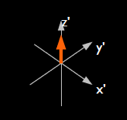
\includegraphics[width=0.5\textwidth]{vite_01}
   \caption{Vector resultante alineado respecto de \Bzero.}
 \label{fig:seq_vectorResultante}
 \end{figg}
\end{figure}

\begin{figure}[htb]
\begin{figg}
   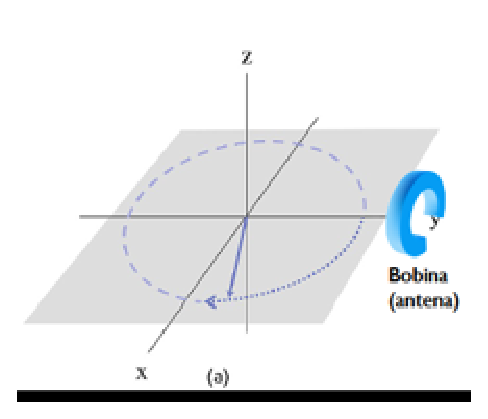
\includegraphics[width=0.5\textwidth]{vite_02}
   \caption{Vector resultante alineado respecto de \Bzero.}
 \label{fig:seq_antena}
 \end{figg}
\end{figure}



Por tanto, para obtener señal de nuestra muestra necesitamos que haya algún vector sobre el eje $x$. Para lograr esto realizaremos un pulso excitador (radiofrecuencia, RF) que cambie la orientación de $M$ del eje $z$ al eje $x$ o plano $x,y$ (es decir \Mz se convierte en \Mxy. Fig \ref{fig:seq_Mx}). Esta perturbación de nuestro sistema inicial permitirá que nuestra antena pueda captar la señal.



\begin{figure}[htb]
\begin{figg}
   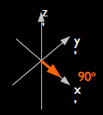
\includegraphics[width=0.5\textwidth]{vite_03}
   \caption{Vector resultante sobre el eje $x$.}
 \label{fig:seq_Mx}
 \end{figg}
\end{figure}


Ahora bien, al apagar el pulso de RF, la señal que hemos recibido irá decayendo debido al fenómeno de relajación transversal. De tal modo que, después de determinado tiempo, podemos decir que $M$ regresará al eje $z$ y volveremos a quedarnos sin señal (fig. \ref{fig:seq_relax}). 

\begin{figure}[htb]
\begin{figg}
   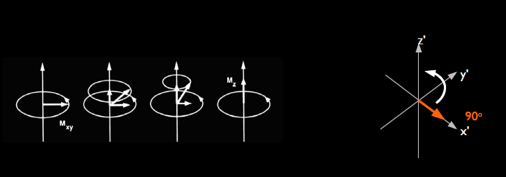
\includegraphics[width=0.75\textwidth]{vite_04}
   \caption{Regreso al estado de reposo.}
 \label{fig:seq_relax}
 \end{figg}
\end{figure}
 


En el proceso que va desde la perturbación de $M$ hasta su regreso al estado de reposo, obtenemos señal a través de la corriente que es inducida en nuestra antena. Cuando $M$ es perturbado y se encuentra sobre el eje $x$, se encuentra precesando y cada vez que pasa por nuestra antena envía electrones. Gracias a este envío de electrones nosotros obtenemos señal. La señal de la que tanto hemos hablado refiere a una onda sinusoide que tiene su mayor amplitud justo después del pulso de RF y que va decayendo conforme pasa el tiempo. El decaimiento se deben enfatizamos, a que el regreso de $M$ al eje $z$ implica una reducción del componente transversal (el único que podemos medir directamente por medio de nuestra antena; fig. \ref{fig:seq_fid}). 

\begin{figure}[htb]
\begin{figg}
   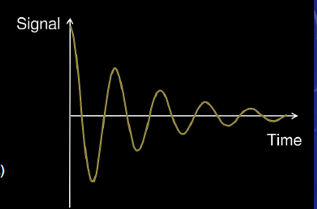
\includegraphics[width=0.5\textwidth]{vite_05}
   \caption{Señal sinusoidal amortiguada.}
 \label{fig:seq_fid}
 \end{figg}
\end{figure}

\section{Secuencias de pulsos generadoras de contraste}

\subsection{Eco de spin}
\index{Eco de spin|textbf}
\index{TE (Tiempo de eco)|textbf}
El eco de spin (SE), como la FID, comienza con un pulso de  RF de 90\degrees. Sin embargo, la diferencia estriba en que agregamos otro pulso de 180\degrees. Lo que lograremos con esto es recuperar la señal que se iba perdiendo con la FID, gracias a un refasamiento de los spins. 

Una vez que hemos realizado un pulso de RF de 90\degrees (fig. \ref{fig:seq_spinecho}-b), el componente transversal de nuestro vector resultante se va reduciendo, debido al desfase de los spins (fig. \ref{fig:seq_spinecho}-c), y por tanto obtenemos menos señal. Una forma de recuperar esta señal es a través de la inducción de un pulso de 180\degrees (fig. \ref{fig:seq_spinecho}-d). 
Cuando realizamos el segundo pulso invertimos el escenario. Los spins se encuentran en una nueva situación (fig. \ref{fig:seq_spinecho}-e) que permitirá que vuelvan a refasarse (fig. \ref{fig:seq_spinecho}-f) y podamos obtener señal. Esta señal recuperada se llama eco y el tiempo que ocurre es proporcional al tiempo entre nuestros pulsos de radiofrecuencia. Precisamente, el tiempo de eco será igual al tiempo transcurrido entre el primer pulso y el eco generado (fig. \ref{fig:seq_TE}).



\begin{figure}[htb]
\begin{figg}
   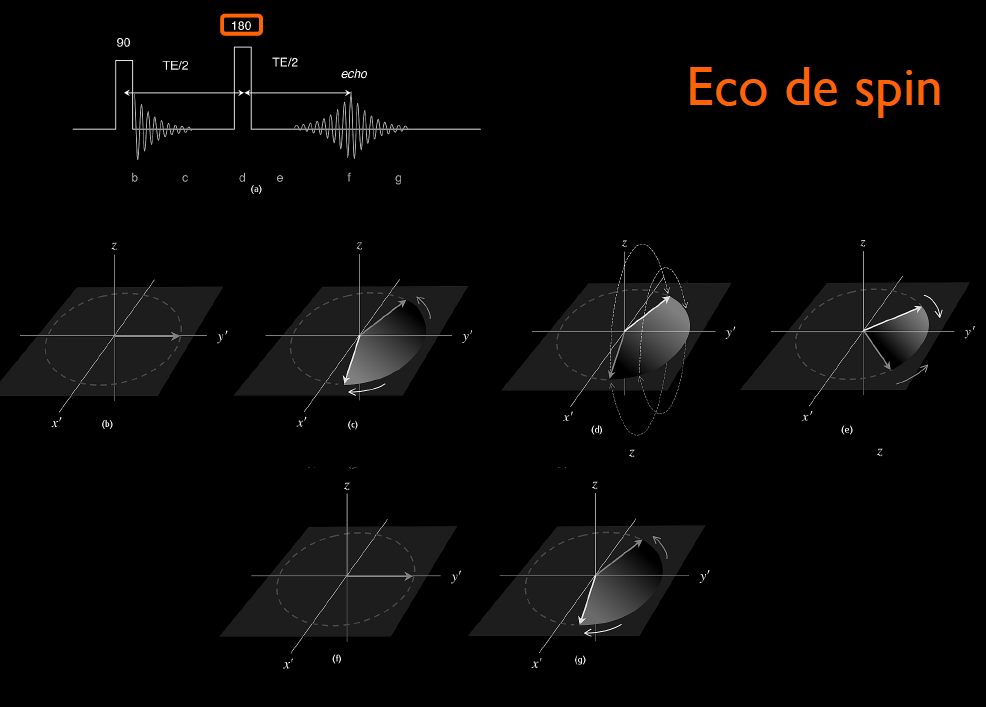
\includegraphics[width=0.75\textwidth]{vite_06}
   \caption{Eco de spin.}
 \label{fig:seq_spinecho}
 \end{figg}
\end{figure}


\begin{figure}[htb]
\begin{figg}
   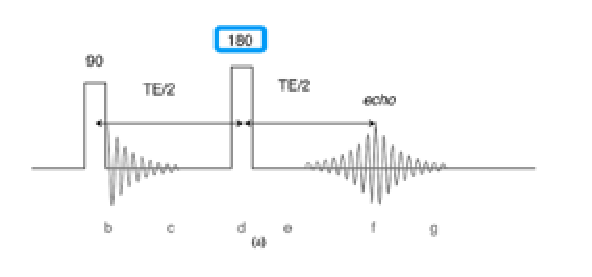
\includegraphics[width=0.75\textwidth]{vite_07}
   \caption{Tiempo de eco.}
 \label{fig:seq_TE}
 \end{figg}
\end{figure}

\subsection{Eco de gradiente }
\index{Eco de gradiente|textbf}
Al igual que el eco de spin, el eco de gradiente (GRE) comienza con un pulso excitador con un ángulo $\alpha$. El ángulo del pulso puede ser de 90\degrees, pero esto dependerá de la información que queramos obtener. Un ángulo de 90\degrees nos permitiría obtener una imagen potenciada a T1, mientras que un ángulo de 10\degrees, podría generar una imagen con información sobre la densidad de protones. 

Después del pulso de RF, se activan dos dos gradientes que nos permitirán generar el eco y la recuperación de la señal correspondiente. El primer gradiente acelera el desfasamientos de los spins. El segundo gradiente tiene la misma amplitud que el primero, pero con signo opuesto. La actividad de este gradiente permite el refase de los spins desfasados inicialmente y la obtención del eco (fig. \ref{fig:seq_GRE}).

Las secuencias con GRE son más rápidas que las generadas por un SE convencional. Sin embargo, la consecuencia de esto son imágenes con mayores artefactos. Esto se debe a que en las secuencias SE, el segundo pulso de 180\degrees ayuda a corregir las heterogeneidades externas. 


\begin{figure}[htb]
\begin{figg}
   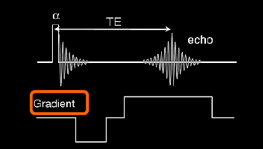
\includegraphics[width=0.75\textwidth]{vite_08}
   \caption{Representación gráfica del eco de gradiente.}
 \label{fig:seq_GRE}
 \end{figg}
\end{figure}


\subsection{Inversión-recuperación}
\index{IR (inversión-recuperación)|textbf}
\label{lab:IR}
El pulso de inversión-recuperación (IR) puede ser considerado un SE convencional, al que se le ha agregado antes un pulso de RF de 180\degrees (fig. \ref{fig:seq_IR}). El tiempo entre el pulso de 180\degrees y el de 90\degrees es conocido como tiempo de inversión (TI), el único cambio que agregaríamos a los parámetros de tiempo presentes en el SE (TE y TR). 


\begin{figure}[htb]
\begin{figg}
   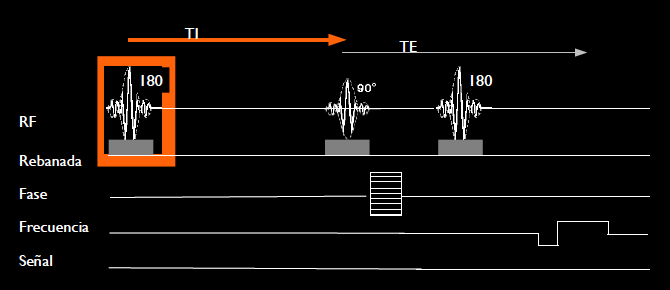
\includegraphics[width=0.75\textwidth]{vite_09}
   \caption{El pulso de inversión-recuperación en una secuencia de pulsos. }
 \label{fig:seq_IR}
 \end{figg}
\end{figure}




La utilidad del pulso IR se ve reflejada en la posibilidad de generar un mayor contraste en imágenes T1 (fig. \ref{fig:seq_RealIR}), así como la supresión de ciertos elementos de nuestra imagen (fig. \ref{fig:seq_supresion}). 

\begin{figure}[htb]
\begin{figg}
   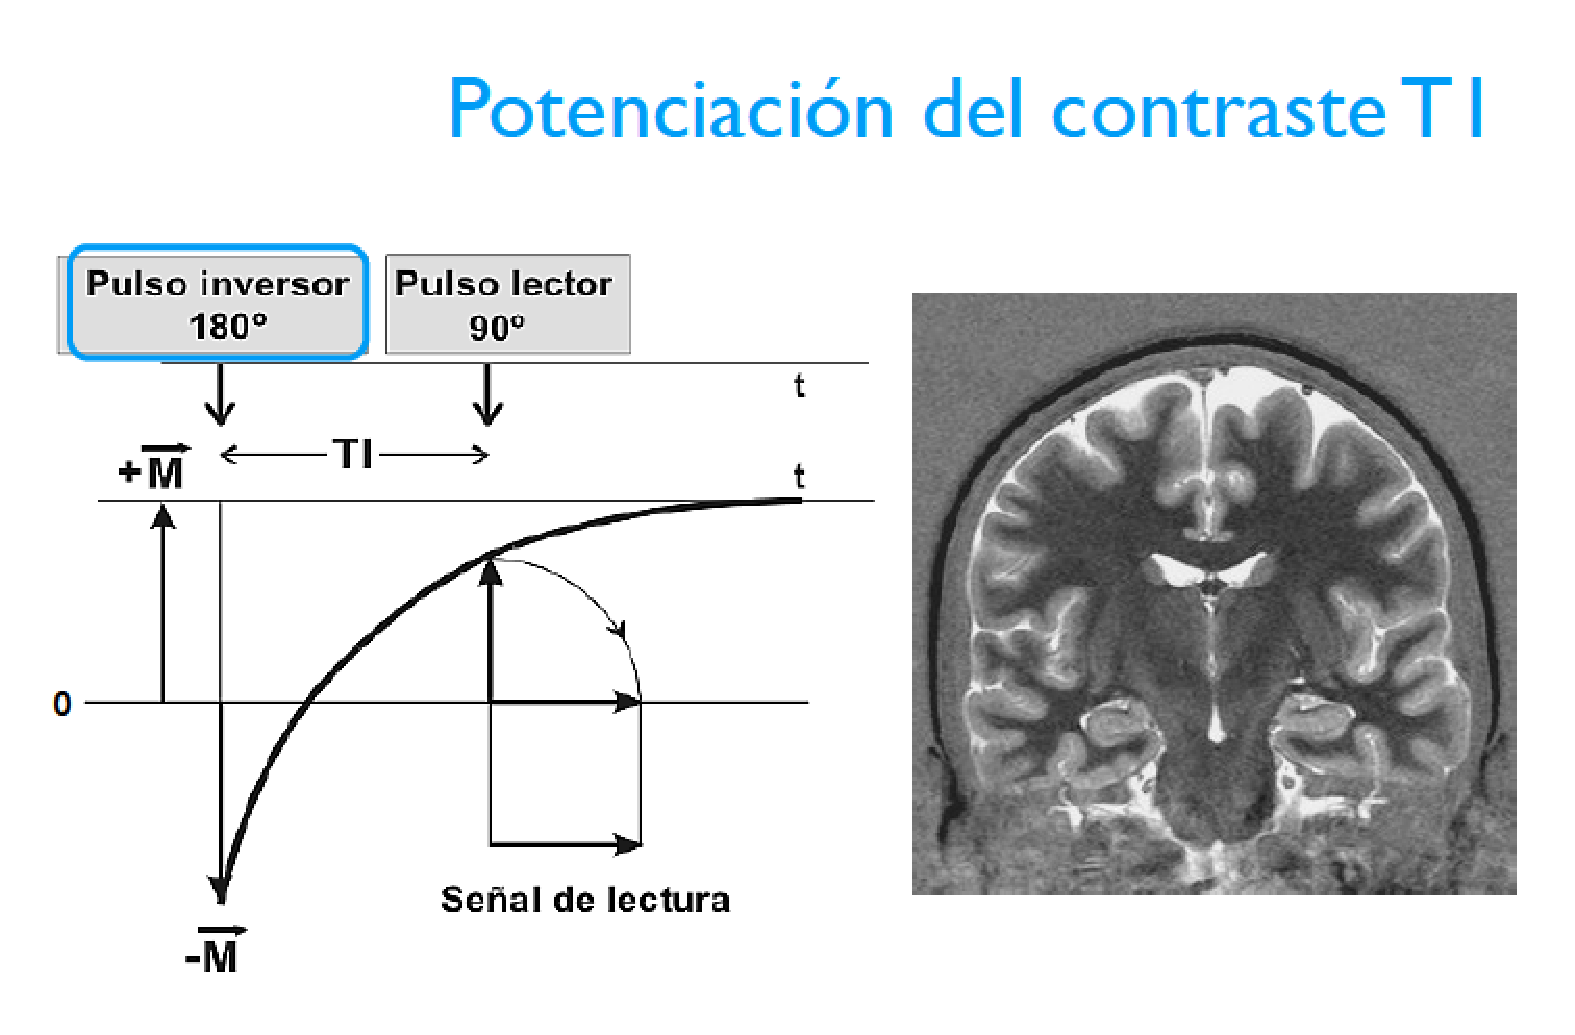
\includegraphics[width=0.75\textwidth]{vite_10}
   \caption{Potenciación del contraste T1 a través de un pulso inversor. En el momento que se aplica el pulso de 90\degrees (pulso lector), las diferencias en el tejido marcadas por TI serán más evidentes gracias al tiempo extra que se ha dado para la relajación de los tejidos.}
 \label{fig:seq_RealIR}
 \end{figg}
\end{figure}

\begin{figure}[htb]
\begin{figg}
   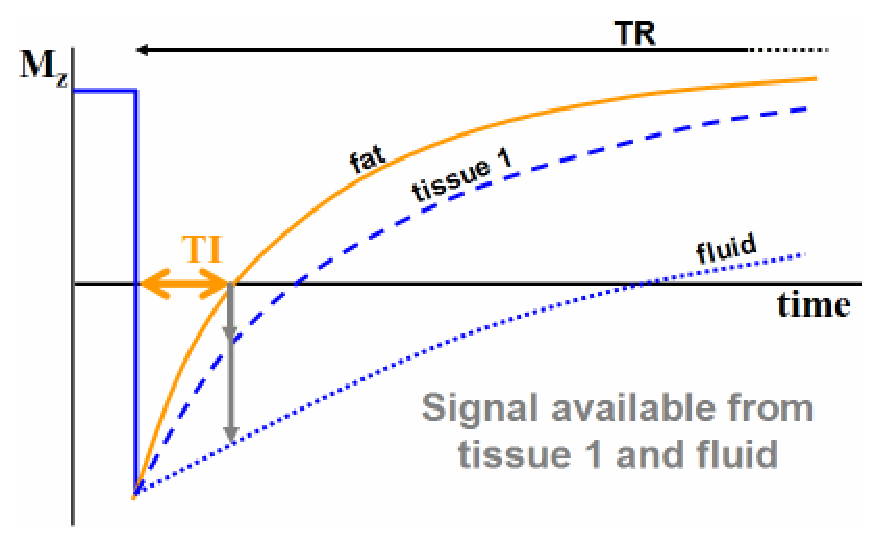
\includegraphics[width=0.75\textwidth]{vite_11}
   \caption{ El TI nos puede ayudar a la supresión de elementos, si conocemos el tiempo de inversión necesario para realizar nuestro pulso lector cuando la señal proveniente de un elemento no tiene presencia sobre el eje $z$. En este caso, la señal de la grasa quedaría suprimida.}
 \label{fig:seq_supresion}
 \end{figg}
\end{figure}




Esta característica del pulso de inversión-recuperación ha ayudado al desarrollo de otras técnicas como FLAIR (\textit{Fluid Attenuated Inversión Recovery})\index{FLAIR|textbf}, que permite la supresión de fluidos (fig. \ref{fig:seq_FLAIR}); y STIR (\textit{Short time inversión Recovery}), la cual permite la atenuación de la grasa (fig. \ref{fig:seq_STIR})\index{STIR|textbf}. En las siguientes figuras podemos encontrar ejemplos de estas herramientas:



\begin{figure}[htb]
\begin{figg}
   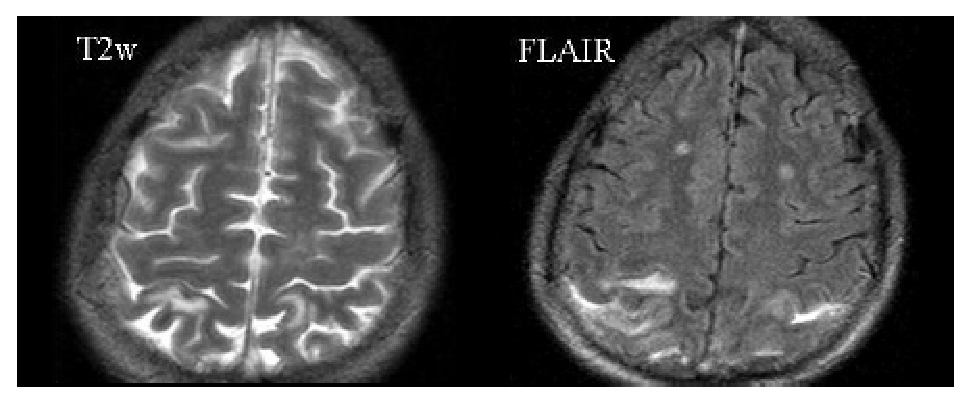
\includegraphics[width=0.75\textwidth]{vite_13}
   \caption{FLAIR. En la parte de la izquierda tenemos una T2 normal. En la imagen de la derecha podemos ver la supresión de las intensidades por FLAIR.}
 \label{fig:seq_FLAIR}
 \end{figg}
 \end{figure}
 
 
\begin{figure}[htb]
\begin{figg}
   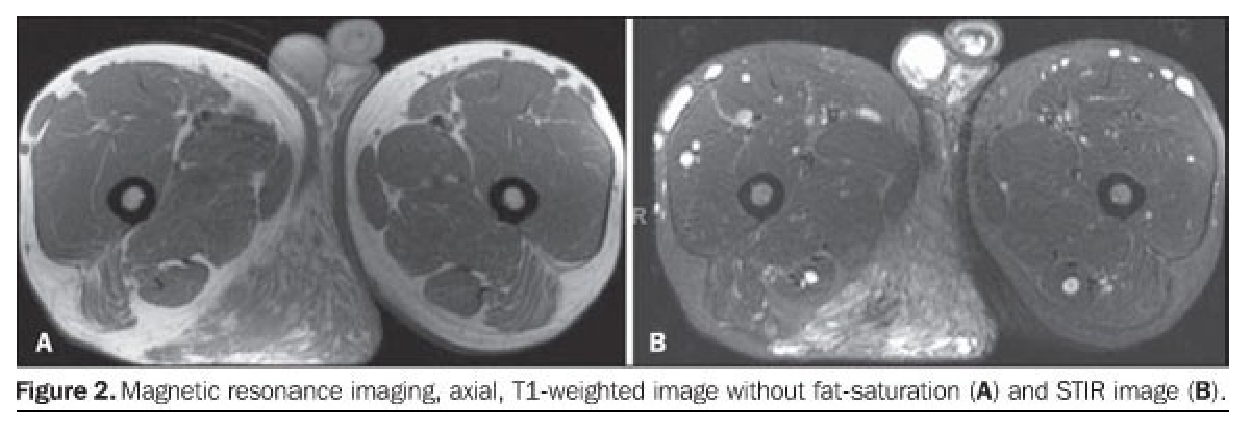
\includegraphics[width=0.75\textwidth]{vite_12}
   \caption{STIR. La imagen de la izquierda es una T1 normal. La imagen de la derecha ha sido obtenida con STIR.}
 \label{fig:seq_STIR}
 \end{figg}
\end{figure}



\section{6.3. Secuencias de pulsos para codificación espacial}

\subsection{Llenado serial del \espaciok}
El llenado serial del \espaciok implica llenar una línea por cada TR, sin saltar líneas, como se muestra en la  figura \ref{fig:seq_kspacelinear}.



\begin{figure}[htb]
\begin{figg}
   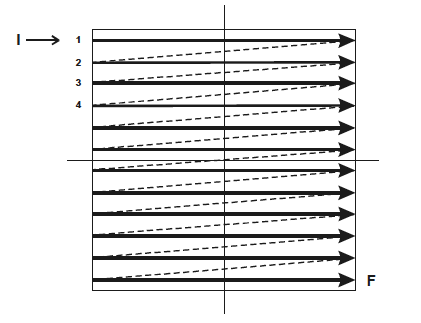
\includegraphics[width=0.75\textwidth]{vite_14}
   \caption{Llenado serial del \espaciok.}
 \label{fig:seq_kspacelinear}
 \end{figg}
\end{figure}


Esta ha sido la forma clásica de llenar el \espaciok. Sin embargo, esto demora mucho la adquisición de imágenes, por lo que nuevas técnicas de llenado del \espaciok han surgido para optimizar los tiempos de obtención. 

\subsection{Secuencias optimizadas para el llenado del \espaciok}
En la actualidad existen técnicas que nos permiten llenar el \espaciok con gran rapidez. Si bien existen una gran variedad de ellas, en esta sección nos enfocaremos a la descripción del turbo-spin eco, el multi-eco y las imágenes ecoplanares. 

\subsubsection{Turbo-spin eco}
\index{Turbo-spin echo|textbf}
El turbo-spin eco (TSE), a diferencia del eco de spin, aprovecha el ``tiempo muerto'', después de la adquisición del eco, para llenar más líneas del \espaciok en menos tiempo, lo cual representa una clara ventaja en comparación con el llenado serial que podemos obtener con una secuencia convencional.
La forma en que se puede lograr esto es a través de un tren de ecos. Después de la secuencia 90-180-eco, es posible el refasamiento de la señal con la introducción de otro pulso de 180\degrees, y así sucesivamente siempre que tengamos señal que recuperar. Para que esto tenga la utilidad deseada resulta necesario hacer un cambio en los gradientes codificadores de fase para que sea posible llenar una línea de \espaciok diferente (fig. \ref{fig:seq_TSE}).


\begin{figure}[htb]
\begin{figg}
   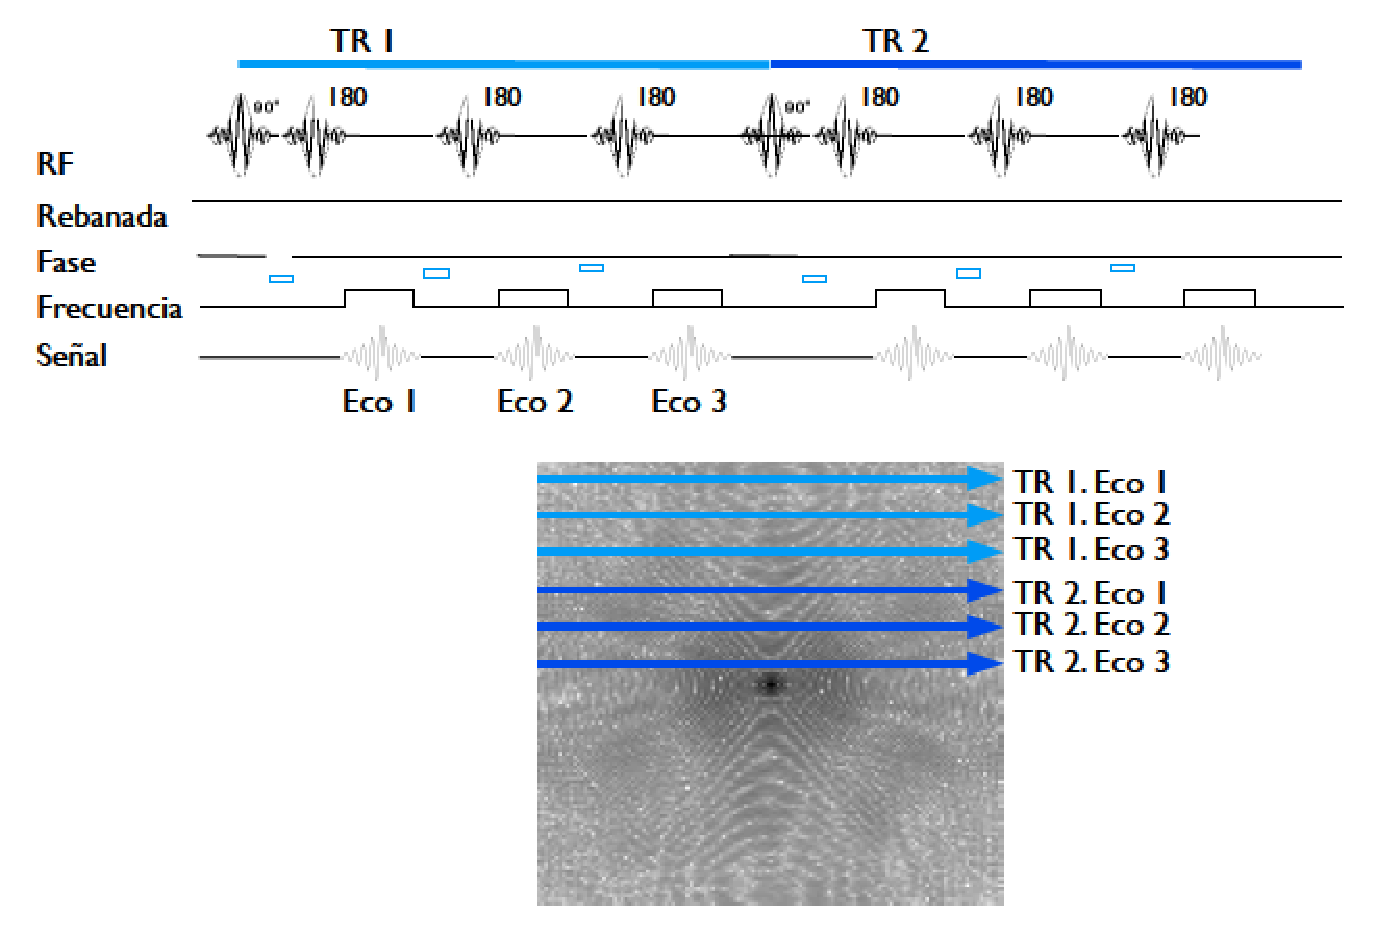
\includegraphics[width=0.75\textwidth]{vite_15}
   \caption{Secuencia turbo-spin eco. En esta secuencia se han llenado tres líneas distintas de \espaciok por cada TR.}
 \label{fig:seq_TSE}
 \end{figg}
\end{figure}




\subsubsection{Multi-spin eco}
\index{Multi-spin echo|textbf}
En el multi-spin eco (MSE) llenamos la misma línea de \espaciok, pero para diferentes imágenes, a diferencia del TSE que llenábamos varias líneas de \espaciok, pero para una misma rebanada.  La ventaja del uso de la secuencia MSE es que podemos ir llenando el \espaciok de imágenes con un distinto contraste, dictado para la diferencia entre los tiempos de eco (fig. \ref{fig:seq_MSE}).



\begin{figure}[htb]
\begin{figg}
   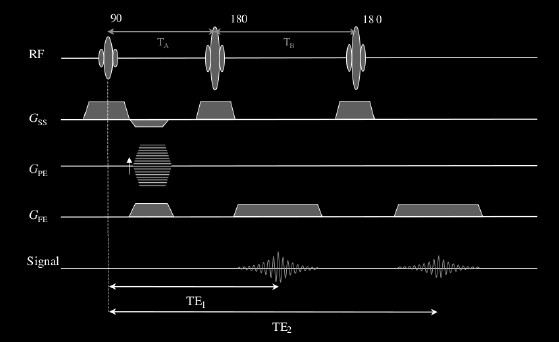
\includegraphics[width=0.75\textwidth]{vite_16}
   \caption{Secuencia multi-spin eco.}
 \label{fig:seq_MSE}
 \end{figg}
\end{figure}



\subsubsection{Imágenes ecoplanares: EPI y multi-shot EPI}
\index{EPI|textbf}
La técnica de imágenes ecoplanares (EPI) es muy poderosa, pues nos permite llenar el espacio-K en un solo TR. Por tanto, podemos tener la información necesaria de nuestra rebanada en un tiempo de adquisición que ronda en los 40 ms.  En la secuencia clásica se parte de un pulso excitador, generalmente de 90. Posteriormente, se generan los ecos necesarios para llenar el \espaciok (fig. \ref{fig:seq_EPI}). El llenado del \espaciok, por otra parte, se ve optimizado al hacerse en zig-zag (16b), debido a que se acorta el tiempo de reposicionamiento de nuestros gradientes. 

Las imágenes obtenidas por EPI nos permiten una adquisición muy veloz. Sin embargo, este factor esta limitado por la atenuación de la señal, con la consiguiente perdida de calidad en nuestras imágenes. Una solución a esto, puede ser llenar el espacio en más de un TR, lo que se conoce como Multi-shot EPI. 


\begin{figure}[htb]
\begin{figg}
   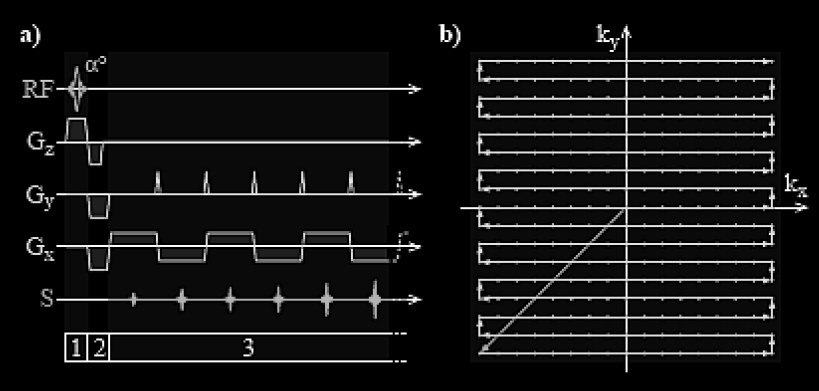
\includegraphics[width=0.75\textwidth]{vite_17}
   \caption{En la imagen de la izquierda se puede apreciar la secuencia de pulsos básica para una imagen ecoplanar. En la imagen de la derecha se muestra esquemáticamente la forma de llenado en zigzag del \espaciok.}
 \label{fig:seq_EPI}
 \end{figg}
\end{figure}




